\normaltrue
\correctiontrue

%\UPSTIidClasse{11} % 11 sup, 12 spé
%\newcommand{\UPSTIidClasse}{11}

\exer{Mouvement RR  $\star$ \label{C2:07:04}}
\setcounter{question}{0}\UPSTIcompetence[2]{B2-14}
\UPSTIcompetence[2]{B2-15}
\UPSTIcompetence[2]{C2-07}
\index{Compétence B2-14}
\index{Compétence B2-15}
\index{Compétence C2-07}
\index{Torseur des actions mécaniques transmissibles}
\index{Torseur d’une action mécanique extérieure}
\index{Principe fondamental de la statique}
\index{PFS}
\index{Mécanisme à 2 rotations}
\ifcorrection
\else
\marginnote{\textbf{Pas de corrigé pour cet exercice.}}
\fi

\ifprof
\else
Soit le mécanisme suivant. On a $\vect{AB}=R\vect{i_1}$ avec $R=\SI{20}{mm}$ et  
$\vect{BC}=L\vect{i_2}$ avec $L=\SI{15}{mm}$. De plus :
\begin{itemize}
\item $G_1$ désigne le centre d'inertie de \textbf{1} et $\vect{AG_1}=\dfrac{1}{2}R\vect{i_1}$, on note $m_1$ la masse de \textbf{1}; %et $\inertie{G_1}{1}=\matinertie{A_1}{B_1}{C_1}{0}{0}{0}{\bas{1}}$; 
\item $G_2$ désigne le centre d'inertie de \textbf{2} et $\vect{BG_2}=\dfrac{1}{2}L\vect{i_2}$, on note $m_2$ la masse de \textbf{2}.% et $\inertie{G_2}{2}=\matinertie{A_2}{B_2}{C_2}{0}{0}{0}{\bas{2}}$.
\end{itemize}

Un moteur électrique positionné entre \textbf{0} et \textbf{1} permet de maintenir \textbf{1} en équilibre.
Un moteur électrique positionné entre \textbf{1} et \textbf{2} permet de maintenir \textbf{2} en équilibre.

L'accélération de la pesanteur est donnée par $\vect{g}=-g\vect{j_0}$.

\begin{center}
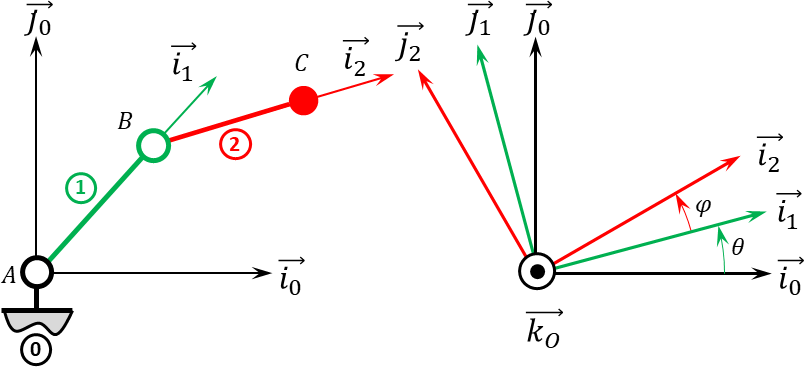
\includegraphics[width=\linewidth]{04_RR_01}
\end{center}
\fi

\question{Réaliser le graphe d'analyse en faisant apparaître l'ensemble des actions mécaniques.}
\ifprof
\begin{center}
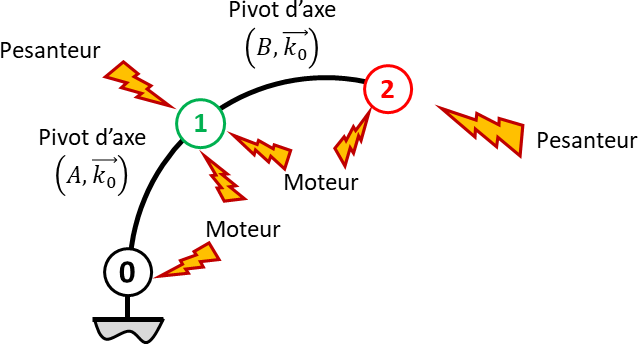
\includegraphics[width=.6\linewidth]{04_RR_01_cor}
\end{center}
\else
\fi


\question{Déterminer le couple à fournir par chacun des moteurs pour maintenir le système à l'équilibre.}
\ifprof
\else
\fi

\ifprof

\question{Donner le torseur de chacune des actions mécaniques.}
\ifprof
\begin{itemize}
\item Pivot entre 0 et 1 : $\torseurstat{T}{0}{1}=\torseurl{X_{01}\vi{0}+Y_{01}\vj{0}+Z_{01}\vk{0}}{M_{01}\vj{0}+N_{01}\vk{0}}{A,\rep{0}}$.
\item Pivot entre 1 et 2 : $\torseurstat{T}{1}{2}=\torseurl{X_{12}\vi{1}+Y_{12}\vj{1}+Z_{12}\vk{1}}{M_{12}\vj{1}+N_{12}\vk{1}}{B,\rep{0}}$.
\item Pesanteur sur 1: $\torseurstat{T}{\text{pes}}{1}=\torseurl{-m_1g\vj{0}}{\vect{0}}{G_1,\rep{0}}$.
\item Pesanteur sur 2: $\torseurstat{T}{\text{pes}}{2}=\torseurl{-m_2g\vj{0}}{\vect{0}}{G_2,\rep{0}}$.
\item Moteur entre 0 et 1 : $\torseurstat{T}{0_{m1}}{1}=\torseurl{\vect{0}}{C_1\vk{0}}{A,\rep{0}}$.
\item Moteur entre 1 et 2 : $\torseurstat{T}{1_{m2}}{2}=\torseurl{\vect{0}}{C_2\vk{0}}{B,\rep{0}}$.
\end{itemize}
\else
\fi

\question{Simplifier les torseurs dans l'hypothèse des problèmes plans.}
\ifprof
\begin{itemize}
\item Pivot entre 0 et 1 : $\torseurstat{T}{0}{1}=\torseurl{X_{01}\vi{0}+Y_{01}\vj{0}}{\vect{0}}{A,\rep{0}}$.
\item Pivot entre 1 et 2 : $\torseurstat{T}{1}{2}=\torseurl{X_{12}\vi{1}+Y_{12}\vj{1}}{\vect{0}}{B,\rep{0}}$.
\item Pesanteur sur 1: $\torseurstat{T}{\text{pes}}{1}=\torseurl{-m_1g\vj{0}}{\vect{0}}{G_1,\rep{0}}$.
\item Pesanteur sur 2: $\torseurstat{T}{\text{pes}}{2}=\torseurl{-m_2g\vj{0}}{\vect{0}}{G_2,\rep{0}}$.
\item Moteur entre 0 et 1 : $\torseurstat{T}{0_{m1}}{1}=\torseurl{\vect{0}}{C_1\vk{0}}{A,\rep{0}}$.
\item Moteur entre 1 et 2 : $\torseurstat{T}{1_{m2}}{2}=\torseurl{\vect{0}}{C_2\vk{0}}{B,\rep{0}}$.
\end{itemize}
\else
\fi

\question{Proposer une démarche permettant de déterminer les couples que doivent développer chacun des moteurs  pour maintenir le mécanisme en équilibre.}
\ifprof
C'est une chaîne ouverte. On isole l'extrémité et on applique le théorème correspondant aux mobilités : 
\begin{itemize}
\item on isole \textbf{2} et on réalise le théorème du moment statique en $A$ en projection sur $\vk{0}$;
\item on isole \textbf{1+2} et on réalise le théorème du moment statique en $B$ en projection sur $\vk{0}$.
\end{itemize}
\else
\fi

\else
\fi




\ifprof
\else
\begin{flushright}
\footnotesize{Corrigé  voir \ref{C1:05:04}.}
\end{flushright}%
\fi